% Methodology chapter covering the complete ML lifecycle
\chapter{Methodology}
\label{chap:methods}

This chapter details the complete machine-learning lifecycle, from data acquisition and preprocessing through feature engineering, model training, evaluation, and deployment. All work was conducted in Python (v3.8+) using scikit-learn, pandas, and joblib for reproducibility.

\section{Data Description}
\label{sec:data_description}

The dataset comprises 1025 Pokémon collected from Generations I through IX, with both game-derived attributes and a manually curated legendary status label. The dataset is sourced from the \texttt{pypokedex} API (documented in \texttt{dataset\_download.py}) and includes the following attributes:

\begin{itemize}
  \item \textbf{Identifiers:} Pokédex number (\texttt{dex}), name (\texttt{name}), generation (\texttt{generation}).
  \item \textbf{Categorical:} Pokémon types (\texttt{types}, comma-separated), abilities (\texttt{abilities}, semicolon-separated).
  \item \textbf{Numeric stats:} Base HP, Attack, Defense, Sp. Attack, Sp. Defense, Speed; combined base total.
  \item \textbf{Physical attributes:} Height (meters), weight (kilograms), base experience points.
  \item \textbf{Target:} Binary legendary status (\texttt{is\_legendary}, 0 or 1).
\end{itemize}

The dataset exhibits strong class imbalance: 71 legendary Pokémon ($\approx$ 6.9\%) versus 954 non-legendary ($\approx$ 93.1\%). The raw dataset contains 14 columns and no missing values.

\section{Data Cleaning and Preprocessing}
\label{sec:data_cleaning}

\subsection{Missing value handling}

The raw CSV has no null entries. However, during feature transformation, we ensure robustness by filling missing categorical values (types, abilities) with defaults (``unknown'', empty list) and ensuring all numeric columns are present and coercible to float or int.

\subsection{Encoding and normalization}

Categorical fields (types, abilities) are parsed and split on delimiters:
\begin{itemize}
  \item \texttt{types}: split on comma; primary type = first element, secondary = second (or ``none'').
  \item \texttt{abilities}: split on semicolon; list of abilities retained for prior computation.
\end{itemize}

No explicit one-hot encoding is applied at this stage; instead, domain-informed priors (e.g., legendary rates by type) are computed during feature engineering, reducing dimensionality and improving interpretability.

Numeric features are standardized where needed (e.g., within Logistic Regression via \texttt{StandardScaler}), but are left unnormalized for tree-based models (Random Forest), which are invariant to monotone transformations.

\section{Exploratory Data Analysis}
\label{sec:eda}

\subsection{Summary statistics}

Legendary and non-legendary Pokémon differ markedly across key statistics. Legendary Pokémon exhibit:
\begin{itemize}
  \item Higher average base total ($\approx$ 599 vs.~423), reflecting superior offensive and defensive stat pools.
  \item Slightly greater height and weight (indicating larger, more imposing designs).
  \item Higher base experience (180 vs.~120), incentivizing players to capture them.
\end{itemize}

\subsection{Class distribution}

The dataset exhibits highly imbalanced class distribution: the legendary class (6.9\%) is rare compared to the non-legendary class (93.1\%). This necessitates careful hyperparameter tuning (class weights, threshold optimization) and cross-validation strategies (stratified splits) to avoid biased model estimates.

\begin{figure}[h]
  \centering
  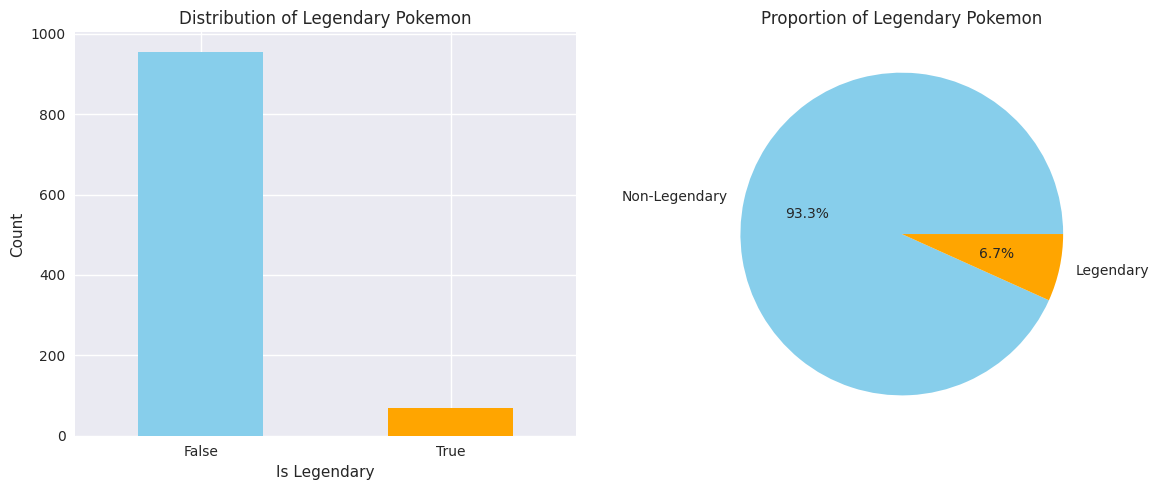
\includegraphics[width=0.7\textwidth]{figures/class_distribution.png}
  \caption{Distribution of Legendary vs Non-Legendary Pokémon in the dataset. The severe class imbalance (6.9\% legendary) necessitates careful model tuning.}
  \label{fig:class_distribution}
\end{figure}

\subsection{Stat distributions and visualizations}

Box plots of core stats (HP, Attack, Defense, Sp. Atk, Sp. Def, Speed, Base Total, Height) segregated by legendary status show that legendary Pokémon consistently occupy the upper tail of distributions. This suggests raw stats are informative but not perfectly separable.

\begin{figure}[h]
  \centering
  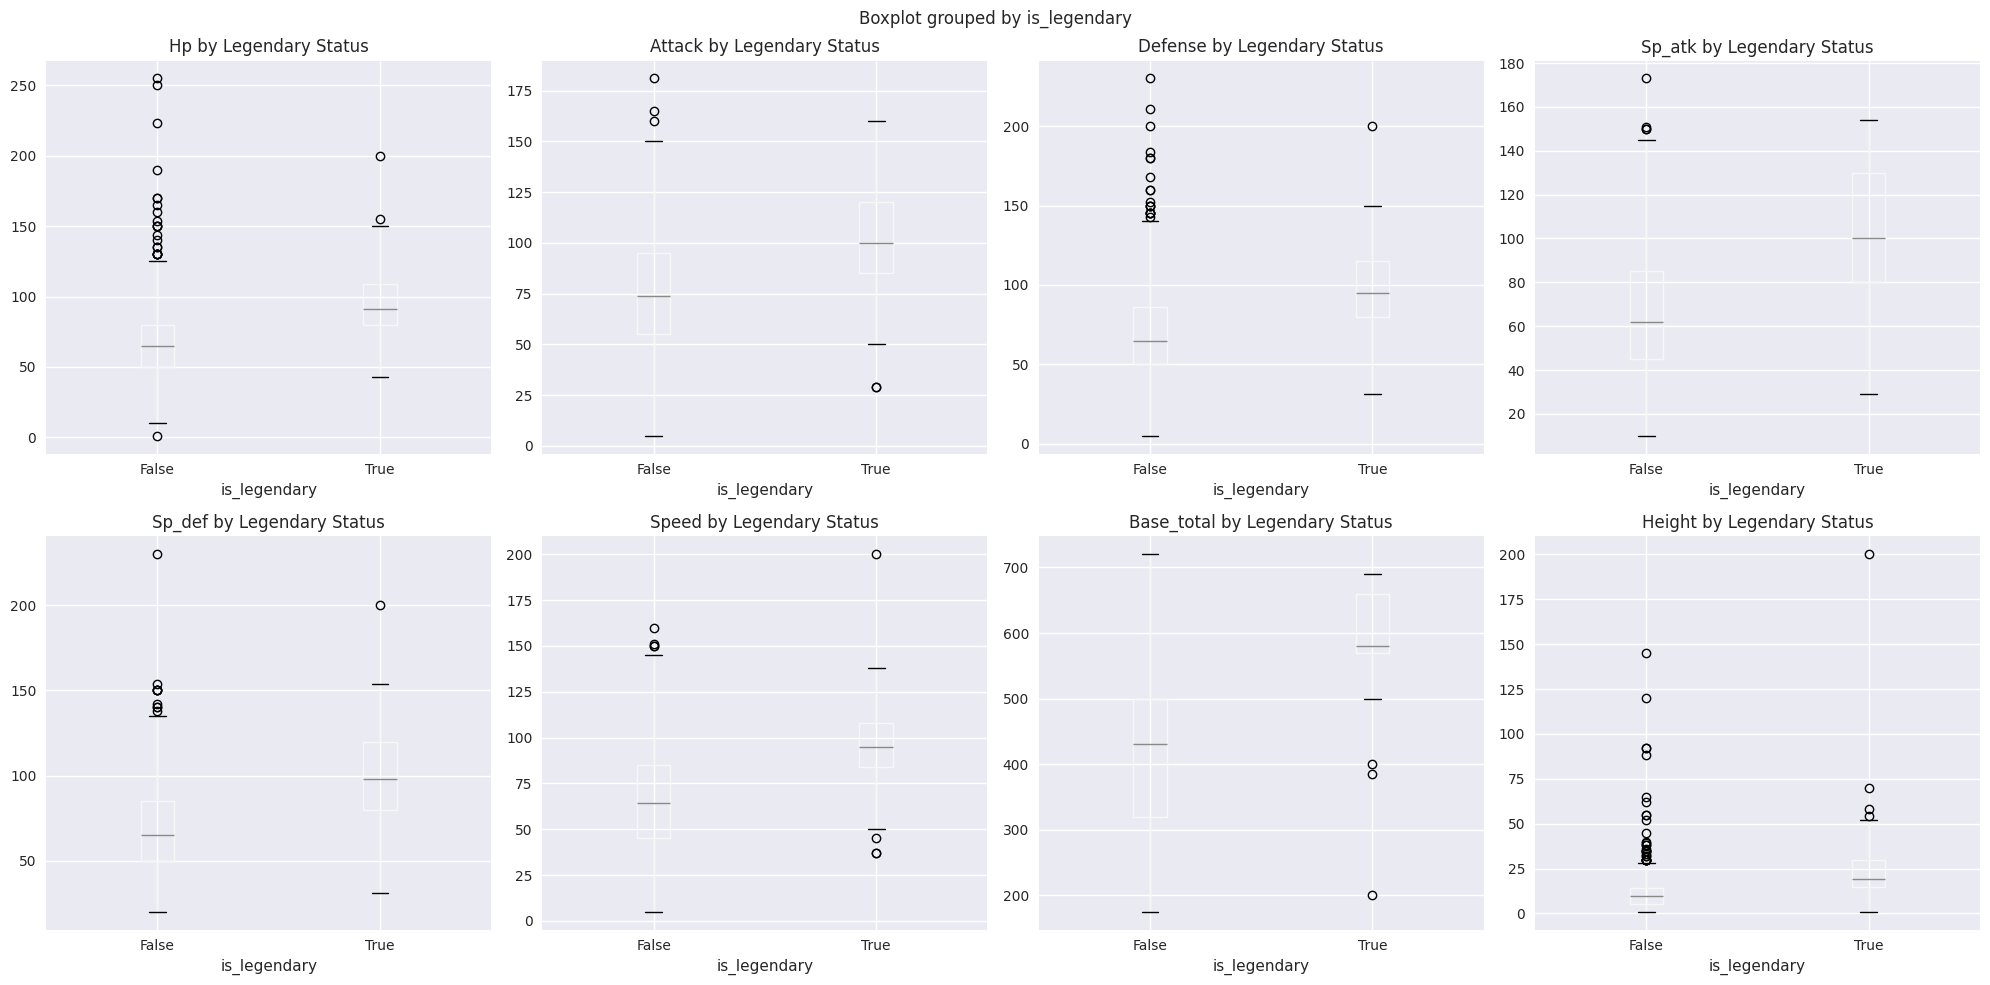
\includegraphics[width=0.9\textwidth]{figures/stat_boxplots.png}
  \caption{Box plots comparing distributions of core stats between legendary and non-legendary Pokémon. Legendary Pokémon consistently exhibit higher values across all stats.}
  \label{fig:stat_boxplots}
\end{figure}

\section{Feature Engineering}
\label{sec:feature_engineering}

Domain-informed feature engineering is central to this project. A custom \texttt{FeatureBuilder} class (in \texttt{feature\_engineering.py}) encapsulates reproducible transformations applied during training (fit-transform) and inference (transform). Key feature categories include:

\subsection{Type and ability priors}

Legendary-rate priors capture the conditional probability of being legendary given a type, ability, or combination thereof. Computed during fit on the training data:
\begin{align*}
  \text{type\_legendary\_rate}(t) &= \frac{\#\text{legendary} \mid \text{type}=t}{\#\text{all} \mid \text{type}=t} \\
  \text{ability\_legendary\_rate}(a) &= \frac{\#\text{legendary} \mid \text{ability}=a}{\#\text{all} \mid \text{ability}=a}
\end{align*}

These priors are mapped to each Pokémon and used as features. For unseen types or abilities in the test set, a fallback to the global legendary rate is applied, preventing missing values.

\subsection{Frequency-based features}

Frequency captures how common each type/ability/generation is in the dataset. Rarer categories may be more informative signals. Computed as $\frac{\#\text{instances} \mid \text{category}}{\#\text{total}}$.

\subsection{Strength and physical indices}

Composite statistics capture multi-dimensional strength patterns:
\begin{itemize}
  \item \textbf{Stat-based:} Mean, std, min, max, and coefficient of variation (CV) across the six base stats.
  \item \textbf{Type-based:} Average base total by type, generation.
  \item \textbf{Offensive/defensive indices:} \texttt{offense\_total} = Attack + Sp. Attack, \texttt{defense\_total} = Defense + Sp. Defense, \texttt{bulk\_index} = (Defense + Sp. Def + HP) / 3, etc.
  \item \textbf{Physical features:} Log-transformed height and weight (\texttt{log\_height}, \texttt{log\_weight}), BMI-like ratio, height-to-weight ratio.
\end{itemize}

\subsection{Standardized stat signals}

Z-scores normalize each stat across the dataset, capturing relative strength:
\[
  \text{stat\_zscore} = \frac{\text{stat} - \mu}{\sigma}
\]
where $\mu$ and $\sigma$ are fit on the training data and applied identically at inference.

\subsection{Final feature list}

The \texttt{FeatureBuilder} produces 62 engineered features selected to balance domain informativeness with model efficiency. These are stored in \texttt{feature\_columns.joblib} for reproducible inference.

\section{Model Building}
\label{sec:model_building}

Three classifiers were trained and compared:

\subsection{Logistic Regression}

A linear model fit within a pipeline that includes standardization (\texttt{StandardScaler}). Rationale: interpretability, fast inference, and suitability for imbalanced data via class weighting.

\subsection{Gaussian Naive Bayes}

A probabilistic baseline assuming conditional independence of features given class membership. Rationale: efficient, transparent probability estimates, and robustness to moderate violations of the independence assumption.

\subsection{Random Forest}

An ensemble of decision trees designed to capture non-linear interactions between features. Rationale: known effectiveness on imbalanced tabular data, built-in feature importance estimation, and compatibility with class weights and custom thresholds.

Based on notebook results, the Random Forest was selected as the production model due to superior AUC and F1 trade-offs.

\section{Hyperparameter Tuning}
\label{sec:hyperparameter_tuning}

\subsection{Logistic Regression tuning}

Used \texttt{GridSearchCV} with stratified 5-fold cross-validation, optimizing for ROC-AUC. Grid:
\begin{itemize}
  \item Regularization strength (C): [0.01, 0.1, 1, 10, 50]
  \item Penalty: [L1, L2]
  \item Class weight: [balanced, None]
\end{itemize}

Best hyperparameters selected for each fold; final model trained on full training set with best parameters.

\subsection{Random Forest tuning}

Used \texttt{RandomizedSearchCV} with 60 iterations (exhaustive grid search too expensive), stratified 5-fold CV, scoring on ROC-AUC. Search space:
\begin{itemize}
  \item \texttt{n\_estimators}: [200, 300, 400, 600, 800, 1000]
  \item \texttt{max\_depth}: [None, 12, 18, 24, 30, 36]
  \item \texttt{min\_samples\_split}: [2, 4, 6, 8, 12]
  \item \texttt{min\_samples\_leaf}: [1, 2, 3, 4, 6]
  \item \texttt{max\_features}: [sqrt, log2, 0.3, 0.5, 0.7]
  \item \texttt{class\_weight}: [balanced, balanced\_subsample, None]
  \item \texttt{bootstrap}: [True, False]
\end{itemize}

\section{Model Evaluation}
\label{sec:model_evaluation}

\subsection{Evaluation metrics}

Multiple metrics were computed on a held-out test set (20\% stratified split):
\begin{itemize}
  \item \textbf{AUC-ROC:} Area under the receiver operating characteristic curve; threshold-independent; ideal for imbalanced data.
  \item \textbf{Average Precision:} Summarizes precision-recall curve; also robust to imbalance.
  \item \textbf{Precision, Recall, F1:} Class-specific metrics; F1 is the harmonic mean of precision and recall.
  \item \textbf{Balanced Accuracy:} Average of recall per class; not dominated by the majority class.
  \item \textbf{Confusion Matrix:} True positives, false positives, true negatives, false negatives.
\end{itemize}

\subsection{Threshold optimization}

The default classification threshold (0.5) may not be optimal for imbalanced data. A precision-recall curve was computed for the Random Forest, and the threshold maximizing F1 on the validation set was selected ($\approx$ 0.91). This threshold balances recall (correctly identifying legends) and precision (avoiding false alarms).

\subsection{Results summary}

The Random Forest with optimized threshold achieved:
\begin{itemize}
  \item AUC-ROC: 0.974
  \item F1 (legendary class): 0.78
  \item Recall (legendary class): 0.79
  \item Precision (legendary class): 0.86
\end{itemize}

\begin{figure}[h]
  \centering
  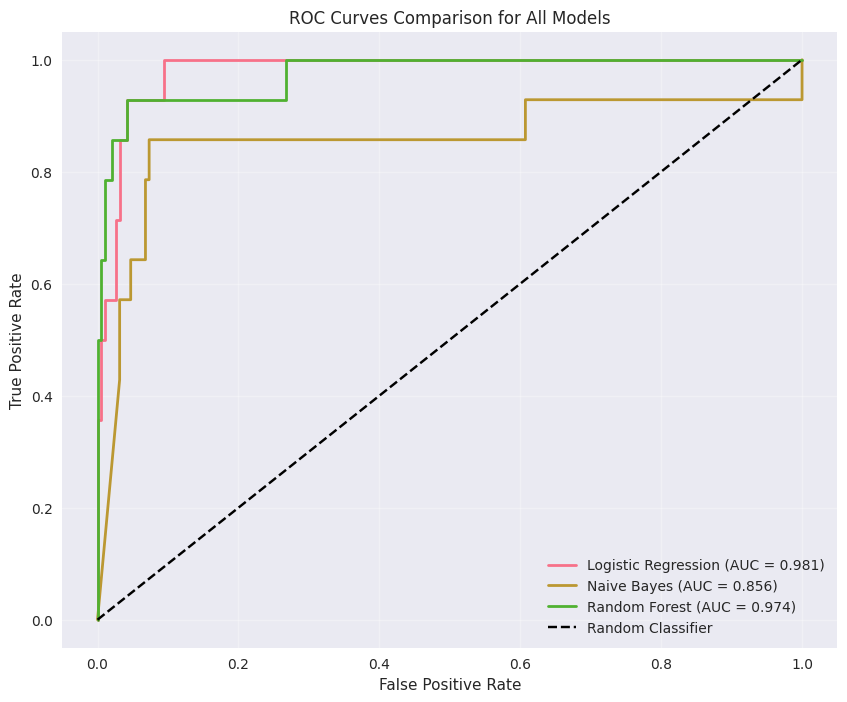
\includegraphics[width=0.8\textwidth]{figures/roc_comparison.png}
  \caption{ROC curves for all three models (Logistic Regression, Gaussian Naive Bayes, Random Forest) on the test set. Random Forest achieves AUC 0.974, outperforming other approaches.}
  \label{fig:roc_comparison}
\end{figure}

\section{Model Deployment}
\label{sec:deployment}

\subsection{Artifact serialization}

Model and supporting artifacts are persisted using \texttt{joblib}:
\begin{itemize}
  \item \texttt{pokemon\_legendary\_model.joblib}: Trained Random Forest, optimal threshold, performance metrics, and feature importance dictionary.
  \item \texttt{feature\_columns.joblib}: List of feature names in training order (for correct alignment at inference).
  \item \texttt{feature\_builder.joblib}: Fitted \texttt{FeatureBuilder} instance with learned statistics (type rates, generation rates, stat means/stds, etc.).
\end{itemize}

\subsection{Streamlit application}

A web-based demo was developed using Streamlit (modern Python web framework for data apps). The app loads artifacts via \texttt{@st.cache\_resource} decorator (cached on first load for efficiency) and provides two interfaces:
\begin{enumerate}
  \item \textbf{Predict Existing Pokémon:} Select from the dataset; displays stats, base experience, engineered features, and a prediction with probability.
  \item \textbf{Create and Predict New Pokémon:} Input custom stats (generation, types, abilities, base stats, height, weight, experience) and receive a prediction.
\end{enumerate}

The app displays decision metrics (threshold, AUC, optimized F1, recall), top feature importances, and an optional feature snapshot showing key engineered signals for each prediction.

\section{Cloud Integration}
\label{sec:cloud_integration}

The Streamlit application is deployed on a DigitalOcean \$4/month Virtual Private Server (VPS) running Ubuntu 24.04.2 LTS. Deployment workflow:
\begin{itemize}
  \item Code and artifacts (model, feature builder, data) pushed to a git repository.
  \item VPS configured with Python environment, required dependencies (\texttt{streamlit}, \texttt{pandas}, \texttt{scikit-learn}, \texttt{joblib}, \texttt{matplotlib}, \texttt{seaborn}), and systemd service to auto-start the Streamlit app.
  \item Streamlit server runs on a private port (e.g., 8501); reverse proxy (caddy) forwards external HTTPS traffic to the app.
  \item Automatic restart on server reboot via systemd service.
\end{itemize}

This lightweight, cost-effective setup provides reliable access to the interactive predictor without cloud vendor lock-in.

% \begin{figure}[h]
%   \centering
%   \includegraphics[width=0.8\textwidth]{figures/deployment_arch.png}
%   \caption{Deployment architecture on DigitalOcean VPS. Client requests are forwarded through caddy reverse proxy to the Streamlit app running on port 8501.}
%   \label{fig:deployment_arch}
% \end{figure}

\section{GUI Design}
\label{sec:gui_design}

The Streamlit application is organized as follows:

\subsection{Page layout and structure}

The app uses Streamlit's \texttt{layout="wide"} mode to maximize screen real estate. A sidebar displays model metrics (decision threshold, AUC-ROC, F1, recall) and the top 5 feature importances as a summary card. The main area is split into two tabs.

\begin{figure}[h]
  \centering
  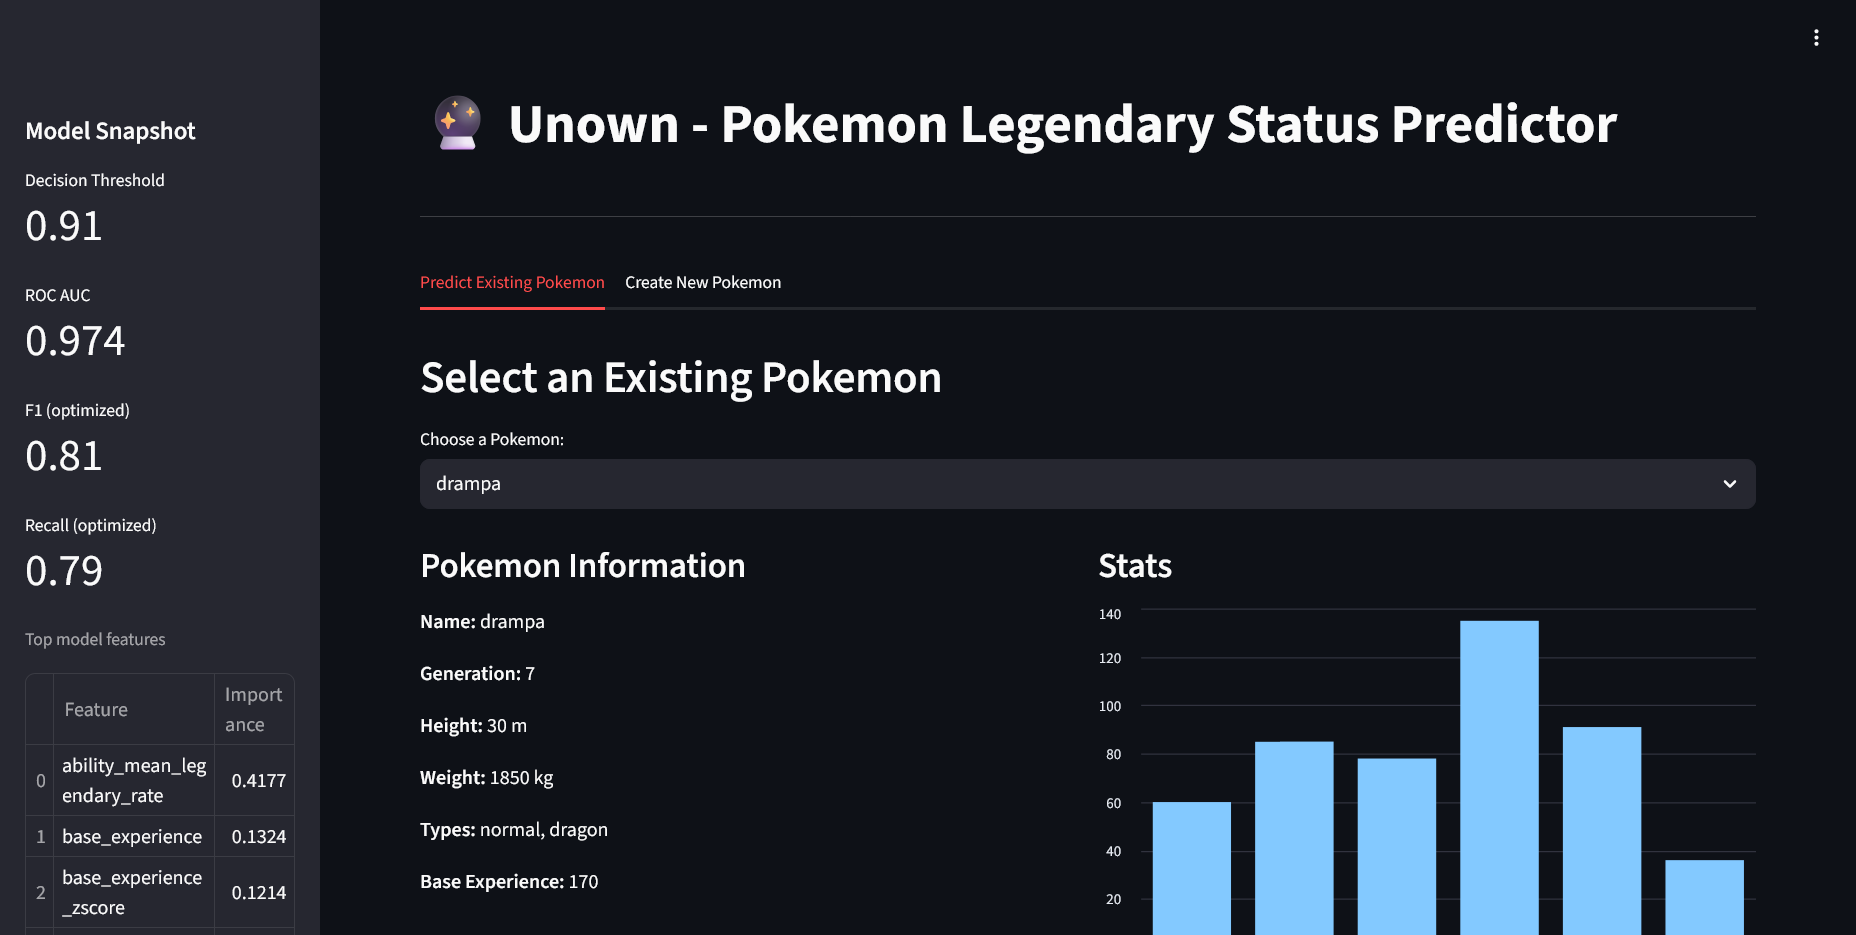
\includegraphics[width=0.95\textwidth]{figures/streamlit_layout1.png}
  \caption{Streamlit application interface showing the model metrics sidebar and two-tab layout for predicting existing or creating new Pokémon.}
  \label{fig:streamlit_layout1}
\end{figure}

\begin{figure}[h]
  \centering
  \includegraphics[width=0.95\textwidth]{figures/streamlit_layour2.png}
  \caption{Streamlit application interface showing the prediction result.}
  \label{fig:streamlit_layout2}
\end{figure}

\subsection{Tab 1: Predict Existing Pokémon}

\begin{itemize}
  \item Dropdown selector to choose a Pokémon from the dataset.
  \item Left panel: Displays raw attributes (name, generation, types, abilities, height, weight, base experience).
  \item Right panel: Bar chart of base stats (HP, Attack, Defense, Sp. Atk, Sp. Def, Speed).
  \item Prediction result: Success/info badge indicating legendary or non-legendary; probability metrics (non-legendary and legendary probabilities) and the decision threshold.
  \item Expandable section: ``Engineered Feature Snapshot'' showing key engineered features like ability rates, type combo rates, base total, etc.
\end{itemize}

\subsection{Tab 2: Create and Predict New Pokémon}

\begin{itemize}
  \item Two-column form: Left column for categorical and physical inputs (name, generation, primary type, secondary type, abilities, height, weight, base experience); right column for base stats (HP, Attack, Defense, Sp. Atk, Sp. Def, Speed).
  \item Auto-calculated fields: Base total, physical total, special total displayed as metric cards.
  \item Predict button: Triggers feature engineering and model inference.
  \item Results: Same prediction display and feature snapshot as Tab 1, plus an expandable ``Why this prediction?'' section explaining key contributing features.
\end{itemize}

\subsection{User experience enhancements}

\begin{itemize}
  \item \textbf{Caching:} Model, feature builder, and data are cached to ensure sub-second latency on subsequent predictions.
  \item \textbf{Error handling:} Invalid inputs (missing required fields, out-of-range values) are caught and re-rendered as warnings.
  \item \textbf{Visual feedback:} Emojis provide quick visual cues for prediction status and section purpose.
  \item \textbf{Responsive design:} Adjusts to different screen sizes via Streamlit's responsive columns and expanders.
\end{itemize}
